\documentclass[%
  a4paper,%
  11pt,% <10pt, 9pt>
  style=print,
  %sender=bottom,
  blue,% <orange, green, violet>
  %rgb, <cmyk>
  %mono,
  bibliography=totoc,
  nexus,
  lnum,
  extramargin
  ]{tubsbook}

\usepackage[utf8x]{inputenc}
\usepackage[english]{babel}
\usepackage{microtype}
\usepackage{graphicx}
\usepackage[hidelinks]{hyperref}
\usepackage{amsmath}
\usepackage{algorithm2e}

% Options for algorithm2e
\RestyleAlgo{algoruled}
\DontPrintSemicolon

% Titlepage 
\subject{Master's Thesis}
\title{Reinforcement Learning for Navigating Particle Swarms by Global Force}
\author{Matthias Konitzny}
\date{\today}
\publishers{\textbf{Institute of Operating Systems and Computer Networks\\ Algorithms Group\\ Prof. Dr. S\'andor Fekete}\\
\vspace*{2em}
Supervisor:\\
Prof. Dr. S\'andor Fekete \par
Dominik Krupke \par}

% Math Operators
\DeclareMathOperator*{\argmax}{arg\,max}
\DeclareMathOperator*{\argmin}{arg\,min}

\begin{document}

\maketitle

\frontmatter

\cleardoublepage
%\makebackpage[plain]%[<plain/info/addressinfo>]


% statement of originality
\thispagestyle{plain} % no header
\vspace*{7cm}
\centerline{\bfseries Statement of Originality}
\vspace*{1em}
\noindent
This thesis has been performed independently with the support of my supervisor/s.
To the best of the author's knowledge, this thesis contains no material previously
published or written by another person except where due reference is made in the text.

\par
  \bigskip\noindent Braunschweig, \today \par
  \vspace*{10mm}
  \hfill\hrulefill
\cleardoublepage

% abstract
\thispagestyle{plain} % no header
\centerline{\bfseries Abstract}
\vspace*{1em}
\noindent
Since the early years of computer science navigation tasks were heavily explored. Since most of these tasks are NP-heavy, even modern computers struggle with the optimal solution of larger instances for those problems. To overcome this problem various approximation algorithms have been developed to get usable results in a relatively short time. In this work we focus on a specific problem: The navigation of particles by a single global force - also known as tilt problem. We exploit recent developments in the area of reinforcement learning to navigate all particles to a given goal position and compare the results to state-of-the-art approximation algorithms. % Running todo
\cleardoublepage

\microtypesetup{protrusion=false}
\tableofcontents
\cleardoublepage

\listoffigures
\cleardoublepage

\listoftables
\cleardoublepage
\microtypesetup{protrusion=true}


\mainmatter
\chapter{Introduction} \label{chp:Introduction}
In this chapter we want to give some introduction into the main focus of this thesis. We start by giving some motivation and historical context on reinforcement learning in Section \ref{sec:Motivation}. We further give an overview over current related work in Section \ref{sec:RelatedWork}, while giving a short summary of our own results in Section \ref{sec:Results}.  

\section{Motivation} \label{sec:Motivation}
\paragraph{History on Machine Learning.}
The idea of intelligent machines which are able to learn more or less autonomously, which are able to solve any complex task by themselves and which thrive for human capabilities or even exceed them was theorized and discussed long before computers were able to learn anything at all. For a long time fiction was way ahead of reality, with films and novels drawing a future of human-like robots - be it positive or negative - while in reality machine learning still struggled at the easiest tasks and was computationally way too heavy to ever run on any machine in a real-time scenario. While we all dreamed of our own Wall-E or feared the rise of Skynet the birth of modern computing not only inspired authors, but also inspired researchers to explore self-learning computers. \\
 This wish to develop intelligent machines found its first success in 1943, when McCulloch and Pitts described how neural networks can be used to build mathematical models for logical or arithmetic expressions \cite{mcculloch1943logical}. With the birth of artificial neural networks, which were introduced in 1959 by Frank Rosenblatt in the form of perceptrons \cite{rosenblatt1958perceptron} a new field of computer science was born. \\
 Even though we had the building blocks to artificial neural networks, there was still a long way before they became as powerful as they are today. Researchers were alternating between breakthroughs and decades of standstill. Even 20 years ago most scientists agreed that artificial neural networks will never become as powerful as other machine learning technologies with stronger mathematical foundations like support vector machines. Today, after the introduction of non-linearity to perceptrons, the breakthrough of the backpropagation algorithm and countless other advances, state-of-the-art models are capable of surpassing humans in a lot of complex tasks like handwriting recognition and are used to solve all kinds of problems where traditional algorithms fail to deliver results. Artificial neural networks developed beyond a point where their capabilities outclass most of the other competing techniques for machine learning and with the ever rising computational power their capabilities only grow further.
 \paragraph{Learning by Doing: Reinforcement Learning} In this work we will be using techniques from a specific sector of machine learning called reinforcement learning or more specifically its modern combination with artificial neural networks called Deep Reinforcement Learning (also \textit{DRL} or Deep RL). \\
 Deep RL is one of the most exciting fields of machine learning today, because it is capable of achieving actual superhuman performance without any human ever creating any training data for it. In reinforcement learning the data is created solely by an agent interacting with its environment. Reinforcement learning can therefore be compared to how humans learn themselves. Therefore all Deep RL algorithms are unsupervised machine learning algorithms. \\ 
 Like traditional machine learning, reinforcement learning has been around for decades, but just recently gained notable attention. In 2013 researchers from the British startup DeepMind were able train a system to play any game from the game console Atari without prior knowledge and only with raw pixel data as input. \cite{mnih2013playing} They later even improved their system and were able to outperform trained human players \cite{mnih2015human}. \\
 But these two successes were only the beginning of a series of advances for deep reinforcement learning. After Google acquired DeepMind their new system \textit{AlphaGo} was able to defeat one of the worlds top class Go players Lee Sedol with 4:1 \cite{borowiec2016alphago} and even the world champion Ke jie in 2017. The system was then expanded and generalized to also play shogi and chess and renamed to \textit{AlphaGo Zero}. AlphaGo Zero not only defeated its predecessor, but also defeated state-of-the-art alpha-beta search engines for chess like Stockfish \cite{silver2017mastering}. In 2019 they reached a new milestone, when their system \textit{AlphaStar} was able to beat a professional player at StarCraft II - a complex multiplayer strategy game \cite{arulkumaran2019alphastar}. \\
We will take an in-depth look of current deep reinforcement learning techniques and how they work in Chapter \ref{chp: RLOverview}.

 \paragraph{Everything can be a Game.}
 We saw reinforcement learning had great success for games, but what happens if we want to solve more abstract problems like wayfinding? Can we still apply these algorithms? The short answer is yes: If we look at it, most algorithmic problems can be easily transformed into a game. We always have something we can express as a state - be it as an actual image or just some numbers - and a well-defined objective for the "player", like finding the shortest path between two points. The player generates the solution for our problem step by step by playing a single round of the "game". \\
 In this work we want to tackle a specific problem: Navigating a swarm of particles to a goal position in a maze-like environment, by applying a global uniform force. This problem finds its application in medicine in form of targeted drug delivery. The goal is to localize medical treatment to efficiently combat cancer, localized infections or internal bleeding, without causing unwanted and potentially harmful side effects for the rest of the body. The delivery requires navigation of the distributed microscopic particles through pathways of blood vessels to a target location. As the particles are too small to build microrobots with sufficient energy to swim against flowing blood, a global external force like an electromagnetic field is used for motion control. This means all particles are subjected into the same direction unless their path is blocked by obstacles. Since at the start all the particles are in different locations, navigating all particles by a uniform force to a single destination is not an easy task. \\ 
 In this work, we want to explore the capability of modern reinforcement learning algorithms on solving this problem. As previous work \cite{becker2020} showed that the problem is NP-hard, finding optimal solutions will not be the goal. Instead we will compare the results to state-of-the-art approximation algorithms. Becker et al. also showed, that reinforcement it is capable of solving this problem for small instances in relatively short time. With this prior knowledge we want to speed up the learning process, aim for larger instances and investigate the possibilities of transfer learning for targeted drug delivery. Our results may also be useful for the application of reinforcement learning on other algorithmic problems.

 \section{Related Work} \label{sec:RelatedWork}
 Some related work. Many nice sources. \\
 Two parts: RL and targeted drug delivery \\
 RL: Large Scale Study, PhD Thesis/Paper
 TDD: Papar, Details on tdd


\section{Our Results} \label{sec:Results}
Hopefully we have some by the time.



\chapter{Reinforcement Learning} \label{chp: RLOverview}
In this chapter we want to give an overview over existing methods for reinforcement learning. RL algorithms can be grouped into multiple families. We provide an overview over some of the most popular methods in Figure \ref{fig:rl_families}. You can see that we have three basic groups of algorithms - the value-based, the policy-based and the model-based methods. Over the years these basic methods were (partially) combined into methods which inherit ideas from multiple basic groups. One the one hand we mainly have variants of the  actor-critic algorithm which all combine value-based and policy-based methods. On the other side we have various combinations of value-based or policy based methods mixed with ideas from the model-based family. For example the earlier mentioned AlphaZero algorithm uses value estimation in combination with \textit{Monte Carlo Tree Search} \cite{silver2017mastering}.

\begin{figure}[ht]
    
  \begin{center}
      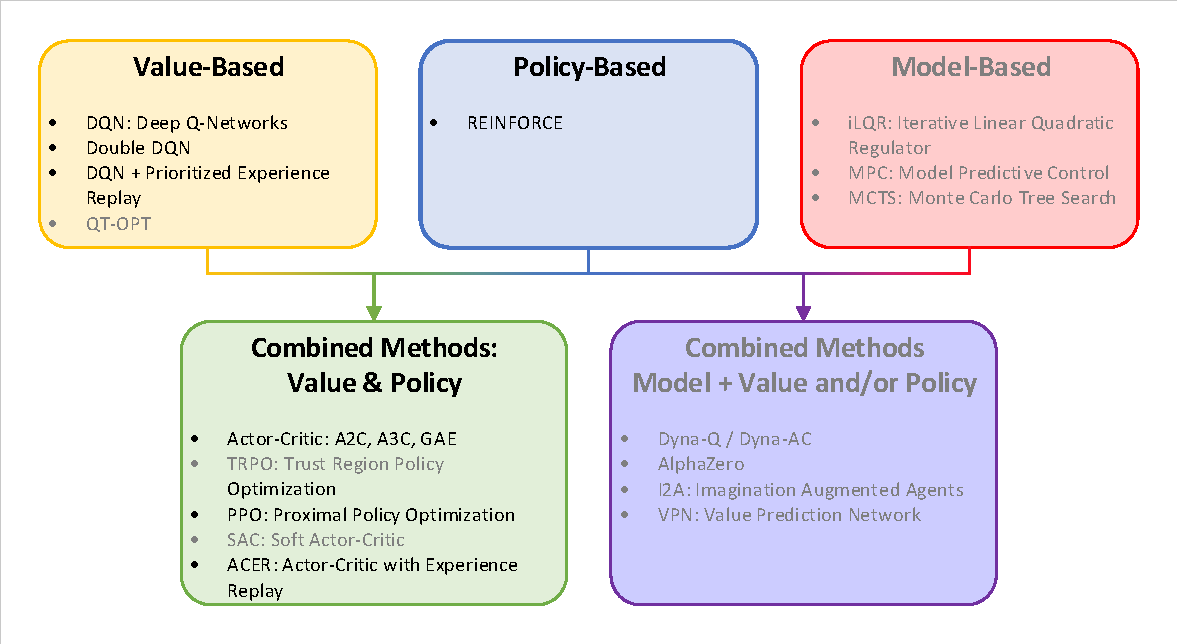
\includegraphics[clip, trim=10px 10px 10px 10px, width=0.95\columnwidth]{figures/rl/rl_families.pdf}
  \end{center}
  
  %\vspace*{-6pt}
  \caption[Overview of RL Families]{Overview of reinforcement learning families (adapted and extended from \cite{foundations2019graesser}). Methods that will not be used in this work are greyed out.}
  \label{fig:rl_families}
  %\vspace*{-12pt}
\end{figure}

In this work we will be focusing on actor-critic variants and value-based algorithms, so we will not cover model-based algorithms here. However we will be taking a look at policy-based methods, since they provide basic building blocks for the algorithms we will be using. \\ 
In this chapter we will begin with some basic ideas and challenges of reinforcement learning, as well as with some mathematical foundations in Section \ref{sec:concepts}. After that we will continue by introducing our first family of RL algorithms the value-based methods in Section \ref{sec:ValueMethods}. We will continue with a short overview over the idea of policy-based algorithms in Section \ref{sec:PGMethods} and will finally cover combined algorithms in Section \ref{sec:CombinedMethods}.


\section{Key Concepts} \label{sec:concepts}
In this Section we give some basic insight into key concepts of reinforcement learning. First we give some basic intuition into how reinforcement learning works and what the challenges are when learning behavior from an unknown environment in Section \ref{ssec:rlidea}. We then continue by defining some of the basic terminology in Section \ref{ssec:rlterms} and finish with a different look on the RL problem from a mathematical point of view in Section \ref{ssec:RLMDP}.  

\subsection{Basic Ideas and Challenges} \label{ssec:rlidea}

Reinforcement learning at its core tries to solve some arbitrary decision-making problem. This problem is given by an \textit{environment} which produces information about its \textit{state} in form of an \textit{observation}. At each timestep an \textit{agent} receives the current observation and then acts according to some \textit{policy} by choosing from a set of available \textit{actions}. These actions should ultimately lead to the achievement of some objective inside of the environment. The behavior of the agent usually is encouraged by some kind of \textit{reward} which is returned by the environment. This basic agent-environment interaction loop is shown in Figure \ref{fig:rl_control_loop} \\ 

\begin{figure}[ht]
    
  \begin{center}
      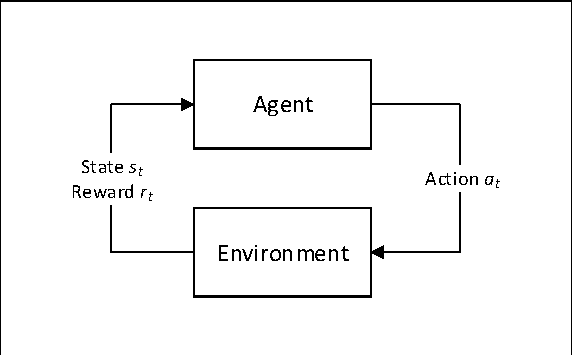
\includegraphics[clip, trim=10px 10px 10px 10px, width=0.6\columnwidth]{figures/rl/rl_control_loop.pdf}
  \end{center}
  
  %\vspace*{-6pt}
  \caption[Agent-environment interaction control loop]{The basic reinforcement learning control loop for agent-environment interaction.}
  \label{fig:rl_control_loop}
  %\vspace*{-12pt}
\end{figure}

This abstract setting can be used to solve a variety of tasks. We have three examples given in Figure \ref{fig:RLExamples}.
\begin{enumerate}
  \item \textbf{Playing the game Breakout.} Breakout is a game from the game console Atari. The goal of the game is to break the bars at the top, by reflecting a moving ball with a paddle at the bottom (like in Ping Pong). The observation is an rgb image of the game itself and the possible actions include resetting or firing the ball as well as moving the paddle to the left or right side of the screen. The reward is the current game score, which increments with every broken piece of barrier at the top. 
  \item \textbf{Playing the game of chess.} The input might be a complex representation of the positions of all pieces, or just a plain rgb-image. The possible actions change after every move, because they are dependent on the valid moves of all pieces. Reward might be as simple as winning ($+1$) or loosing ($-1$) the game, but can be more complex.
  \item \textbf{Grasping objects in a container.} A robotic arm should be trained to grasp arbitrary objects in a container. The observation is a plain image captured from above the robotic arm and a positive reward is given if the robot is able to successfully grasp an object. Actions include positioning the robot arm and opening or closing the "hand". 
\end{enumerate}

\begin{figure}[ht]
  \begin{center}
  \resizebox{0.95\columnwidth}{!}{%
  \begin{tabular}{ccc}
    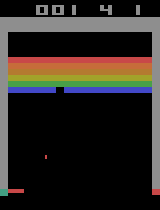
\includegraphics[clip, height=5cm]{figures/rl/Breakout.png}  &
  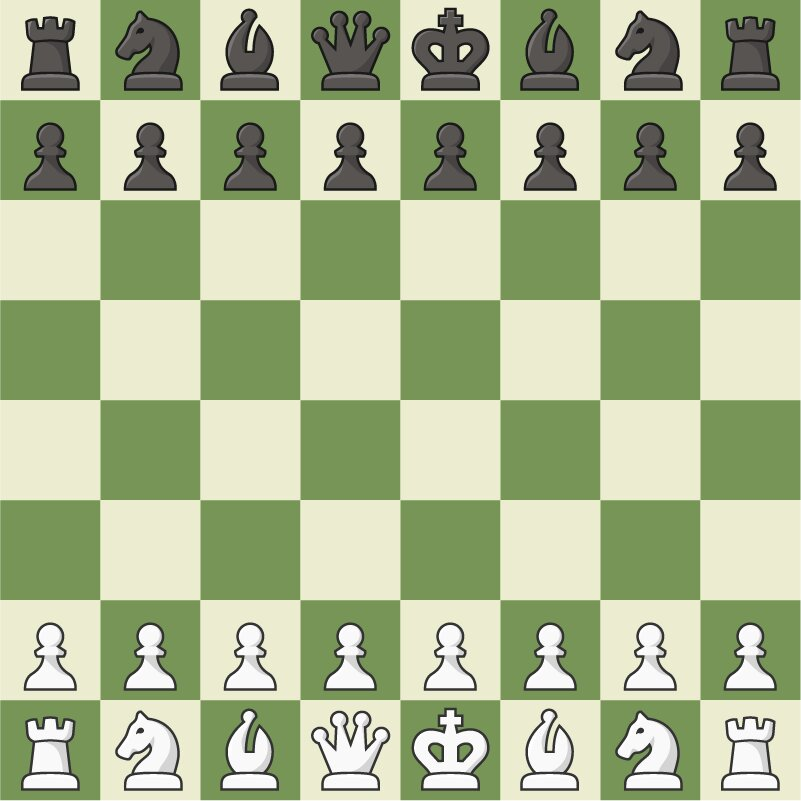
\includegraphics[height=5cm, keepaspectratio]{figures/rl/chess.jpg} & 
  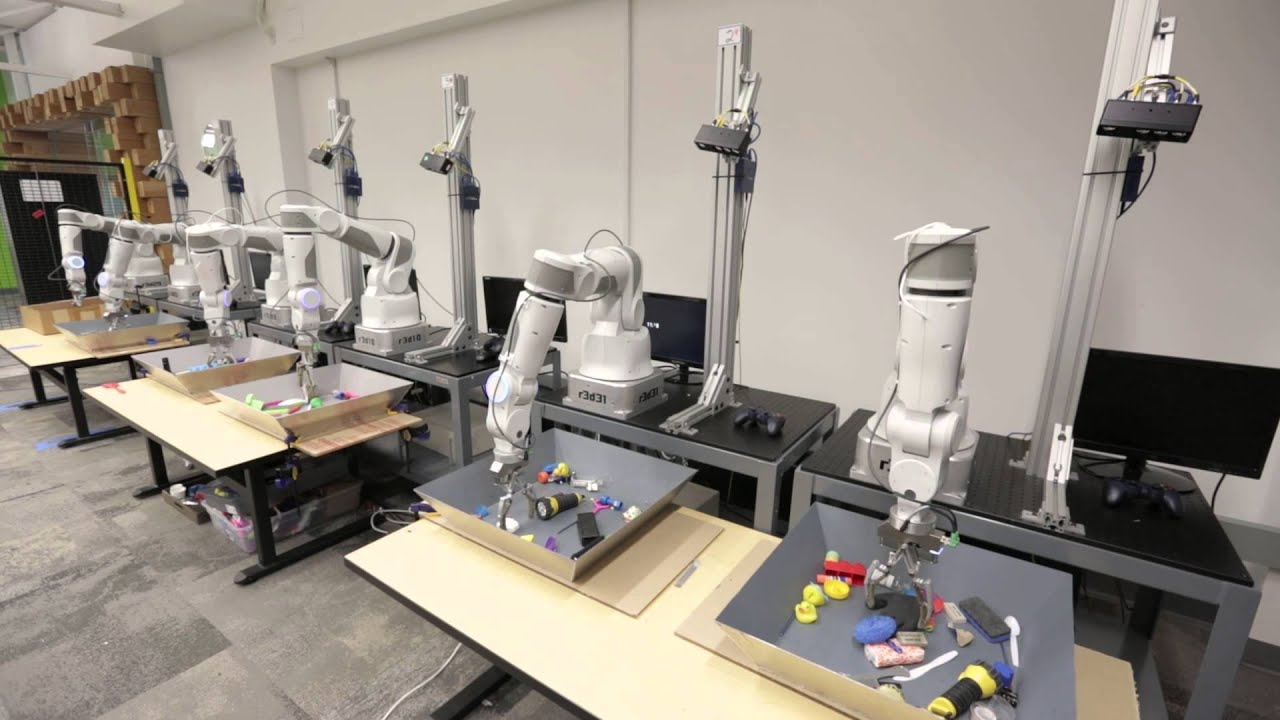
\includegraphics[trim=400px 0px 75px 0px, clip, height=5cm, keepaspectratio]{figures/rl/Google_Robot_Learning.jpg}\\
  {(a) The Atari game Breakout} &
  {(b) Chess\footnotemark} &
  {(c) Google Robot Grasping \footnotemark}\\
  
  \end{tabular}
  }%
  \end{center}
  %\vspace*{-12pt}
  \caption{Reinforcement learning examples.}
  \label{fig:RLExamples}
  %\vspace*{-12pt}
\end{figure}
  
\footnotetext{Image from chess.com \url{https://www.chess.com/bundles/web/images/offline-play/standardboard.6a504885.png}}
\footnotetext{Image from ai.googleblog.com \url{https://i.ytimg.com/vi/iaF43Ze1oeI/maxresdefault.jpg}}

Let's take a closer look at another example, pictured in Figure \ref{fig:CartPole}: The game of balancing a stick on a cart in a 2D environment. The sick can only be balanced by moving the cart, which has some velocity and can either be accelerated to the left or to the right. At each timestep the agent gets an observation which describes the current position and angle of the sick and can then choose which action it wants to take. If the stick falls over the agent looses. If it is able to balance the stick for more than 200 steps it wins. At each step it survives it gets a reward of $+1$. \\
Balancing a stick is harder than it initially seems to be. A simple algorithm which always moves the cart towards the direction the stick is leaning to, will always overshoot after a short time and loose balance. Of course we can think of a more complex algorithm and maybe solve the problem this way, but what if we want the computer to figure things out? How can we implement an algorithm which figures out on its own which actions should be taken for some given observation? How would we ourselves solve this problem? The answer is simple try and error. A human learns how to balance a stick, by balancing it. This will of course fail at the beginning, but after some time a human would get better and better at \textit{estimating} how the stick behaves in response to the actions that were taken. Similarly our reinforcement learning algorithm should just play around and looks at the results. Did the stick fell over? How long were we able to balance the stick? At which point did it fell and which actions led to that outcome? If we can answer all these questions we might be able to learn how to solve the problem. \\

\begin{figure}[ht]
  
  \begin{center}
      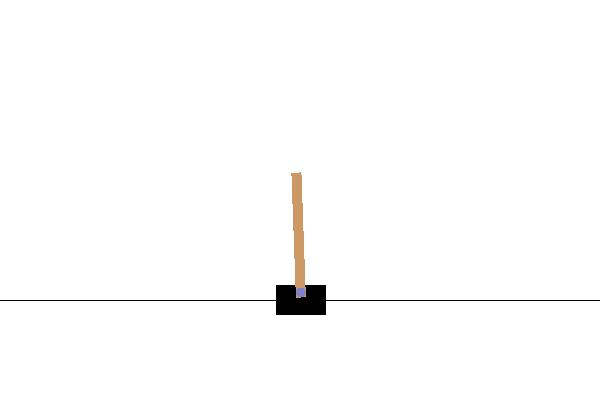
\includegraphics[trim=0px 50px 0px 100px, clip, width=0.6\columnwidth]{figures/rl/CartPole.jpg}
  \end{center}
  
  %\vspace*{-6pt}
  \caption[CartPole Environment]{A classic toy example from OpenAI gym \cite{openAIgym}: The CartPole environment.}
  \label{fig:CartPole}
  %\vspace*{-12pt}
\end{figure}


Building an association between some action and the resulting outcome in the environment is actually one of the greatest challenges for RL algorithms and known as the \textit{credit assignment problem}. Since rewards are typically sparse and delayed, understanding their origin is hard. Especially if you think about more complex games like chess, it is really unclear to what extend which move was responsible for winning or loosing a game. This problem becomes even greater the more sparse the rewards get: If we only reward winning or loosing, figuring out what made us win or loose is pretty hard, but if we reward or punish every single action, we might end up with a copy of an already known strategy. The challenge is to create an unbiased reward signal which does not distort the learning process. In the case of balancing a stick this is easy. Balancing the stick for a longer time is always good and can be rewarded. But as problems become more complex it is unclear if an action is actually good. If we take another look at chess for example, it might be beneficial to take a piece of your opponent, but it might also be better to go for a check or something which just gives you a positional advantage. Which action should be rewarded to what extend? In the end it is also a balance with how much time there is to learn. Sparse rewards will always result in longer training times, but give more freedom and thus might yield better results. \\
In the presence of sparse rewards another challenge arises: What if our learning algorithm is not able to find any solution at all? How can the algorithm know that there is a better solution out there, than the solution it already found? The answer is it cannot. The observations the agent makes in the environment are dependent on the taken actions. If the agent chooses the wrong actions it might never be able to explore the environment to a point where it receives more reward. The agent might get stuck with the false impression that it already achieved the maximum reward that is possible. \\
The last challenge we want to talk about is closely connected to the second one: Keeping the balance between exploration of the environment and exploitation of already learned behavior. Often diverging from already proven behavior decreases the short-term reward, but might lead to a much larger reward in the future. People face this problem in their everyday life: If you know the route from your home to some place, you are way more likely to take that route, than trying to find a shorter one, but risking the eventual failure. In this scenario the person - or in RL the agent - might get stuck in a situation where it never does anything else than taking the best known route, and get forever stuck in this local optimum.

\subsection{Terminology} \label{ssec:rlterms}
We already talked a lot about the existing challenges of reinforcement learning. Before we want to dive deeper into the various techniques that were developed to overcome these problems, we want to take a short look on the common terminology used throughout these algorithms.

\paragraph{States and Observations.}
For every environment there is a difference between the internal state $s$ of the environment and the observation $o$ an agent receives. While the state covers all information about the "world" the environment represents, the observation is a representation of that world and may or may not contain all information. Depending weather we can observe the whole environment or not, we talk about fully or partially observed environments. Observations are typically given to the agent as a real-valued vector. 

\paragraph{Actions.}
Actions are the things an agent can do in the environment. Most of the time they are fairly simple, like deciding to go left or right, but they can be more complex. \\
The set of actions an agent can perform in an environment is usually called the \textit{action space}. Depending on the environment, the action space might be discrete - with only a finite number of available choices - or continuous. Discrete action spaces are typical for game-like environment like CartPole or Breakout. Usually discrete actions are mutually exclusive, meaning only a single action can be chosen at a time: We can not go left and right - we have to choose. \\
Continuous action spaces on the other hand allow for a value attached to each available action and are often found in robot control tasks. For example if we look at a self-driving car, we have an action for the degree of the steering wheel and an action for the position of each pedal which need to be set in each step. \\
Not all RL algorithms are able to handle both types of action spaces. In some instances it is possible to transform continuous action spaces into discrete action spaces if no absolute precision is necessary. However this often results in a very high number of available actions.

\paragraph{Policies.}
Most of the time the words agent and policy will be used in the same manner. For the sake of clarity we want to define the policy as the rule(s) an agent uses to decide which action should be taken for some observation. We can think of the policy as the actors brain. \\
We denote the policy by $\mu$ if it is deterministic and $\pi$ if it is stochastic. Later when we are focusing on deep RL all of our policies will be build from artificial neural networks which are parameterized by their weights and biases. We therefore extend our notion to include these parameters as $\theta$ to have parameterizable policies $\mu_\theta$ and $\pi_\theta$. If the agent receives an observation at time $t$ it then generates the action according to its policy by:
\begin{align*}
  a_t &= \mu_\theta(o_t) \\
  a_t &\sim \pi_\theta(o_t)
\end{align*}


\paragraph{Episodes and Trajectories.}
We define an episode as a single run of an environment. So for chess an episode is a single game an agent played. While the agent played the episode it generates a \textit{trajectory} $\tau$, which is a sequence of triples from (state, action, reward), describing the episode:
\[\tau = ((s_0, a_0, r_0),  (s_1, a_1, r_1)) \]
The initial state of the environment is randomly sampled from some start-state distribution $\rho_0$. State transitions $s_t \rightarrow s_{t+1}$ happen according to the laws of the environment and the chosen action: $s_{t+1} = f(s_t, a_t)$. An episode might be infinitely long depending on the environment, which also leads to an infinite trajectory. In literature the words episode, trajectory and rollout are often used in a very similar fashion. 


\subsection{Reinforcement Learning as Markov Decision Process} \label{ssec:RLMDP}
In this section we want to take a look at the theoretical foundations of reinforcement learning. We will do this by looking at how we can model every RL problem with a discrete action space as a \textit{Markov Decision Process}. MDPs provide a mathematical framework for decision making processes and were introduced in the 1950s by Richard Bellman \cite{bellman1957markovian}. They were named after an earlier model the \textit{Markov Chains} which were created by the mathematician Andrey Markov who studied stochastic processes without memory. In this section we will see how MDPs build the foundations of value-based RL algorithms. \\
Before we talk about MDPs, let us take a step back and first talk about Markov Chains. In Markov Chains we have a fixed number of \textit{states} and \textit{transition probabilities} which define how likely it is to move from one state to another. We start in a given state and at each step the system randomly evolves from one state $s$ to another state $s'$. This transition only depends on the states' transition probability and is not related to earlier transitions. This is called the \textit{Markov Assumption}. Figure \ref{fig:MarkovChain} shows an example of a Markov Chain. \\

\begin{figure}[ht]
  
  \begin{center}
      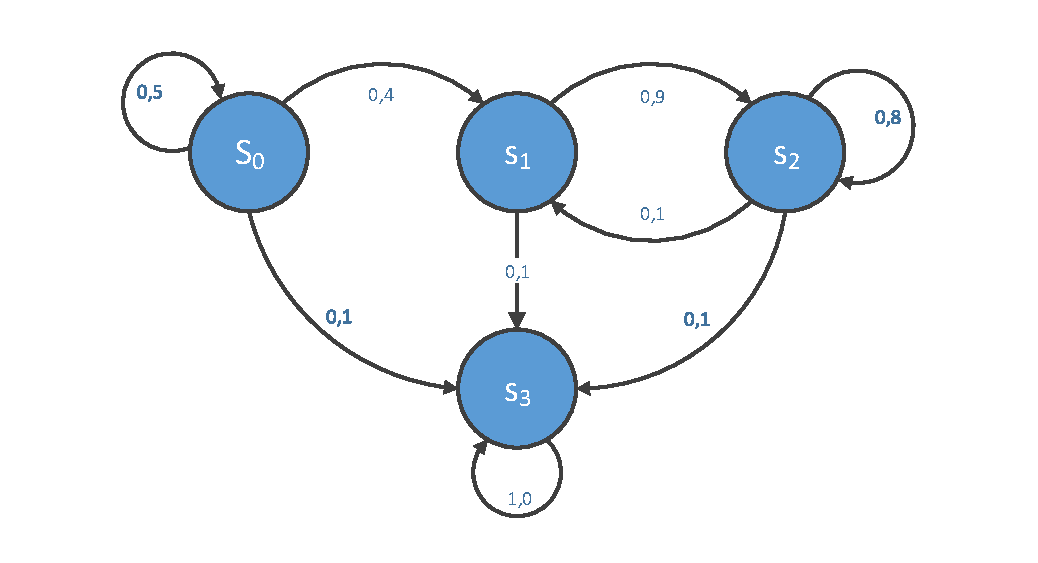
\includegraphics[trim=10px 10px 10px 10px, clip, width=0.8\columnwidth]{figures/rl/markov_chain.pdf}
  \end{center}
  
  %\vspace*{-6pt}
  \caption[An Markov Chain Example]{An example for a Markov chain. Suppose we start in $s_0$. There is a 50\% chance of staying in that state, a 40\% chance of transitioning to $s_1$ and a 10\% chance of transitioning to $s_3$. No matter how long it alternates between $s_0$, $s_1$ or $s_2$ at some point it will enter $s_3$ and remain there forever, because $s_3$ has a 100\% chance of transitioning to itself.}
  \label{fig:MarkovChain}
  %\vspace*{-12pt}
\end{figure}


Markov decision processes extend the idea of Markov chains with an active agent. At each step, the agent can choose from a set of actions and the state transition probability depends on the chosen action. Additionally each state transition may return some reward. The agents goal is to find a policy which maximizes the total reward over time. We extended our example from Figure \ref{fig:MarkovChain} with actions and rewards in Figure \ref{fig:MDP}. Like for Markov Chains, MDPs transition probabilities must only depend on the current state $s$ and the chosen action.\\

\begin{figure}[ht]
  
  \begin{center}
      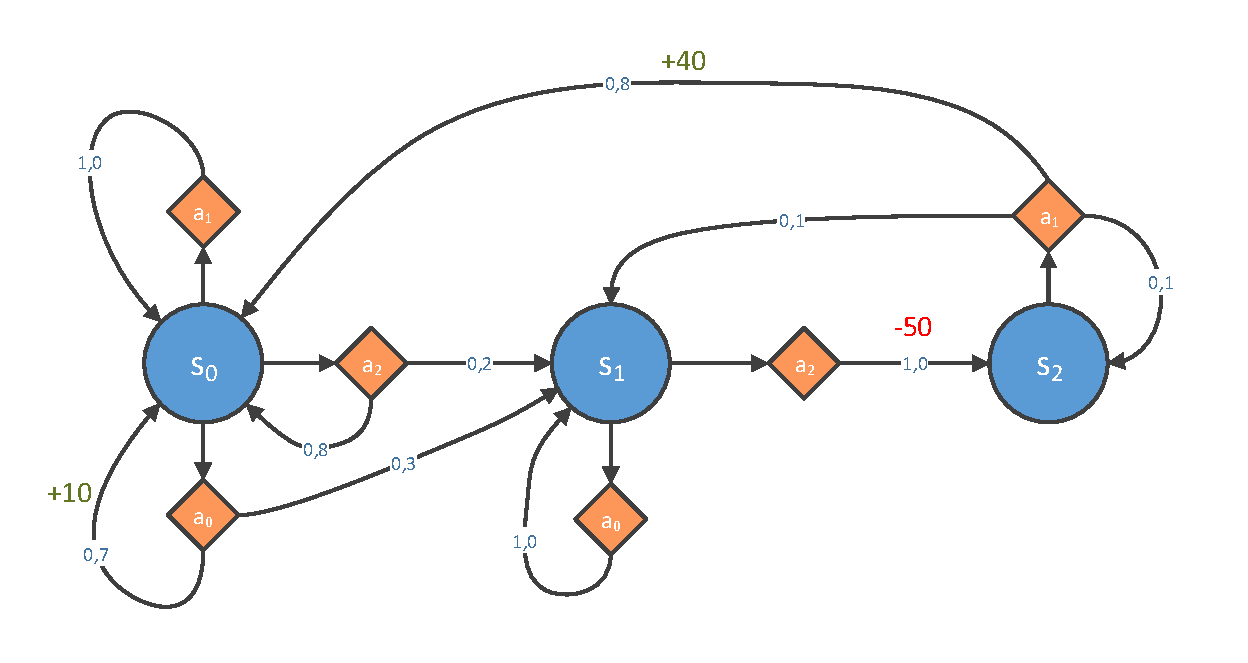
\includegraphics[trim=10px 10px 10px 10px, clip, width=0.9\columnwidth]{figures/rl/markov_decision_process.pdf}
  \end{center}
  
  %\vspace*{-6pt}
  \caption[An Example for the Markov Decision Process Example]{An example for the Markov decision process (recreated from \cite{handson2019geron}). Again we start in $s_0$ and the agent can choose from the actions $a_0$, $a_1$ or $a_2$. Choosing $a_0$ will give it a reward of $+10$. With a probability of 70\% the agent will be staying in $s_0$ and with a probability of 30\% it will transition to $s_1$. So the agent can likely repeat action $a_0$ in $s_0$ multiple times, but will at some point transition to $s_1$. In $s_1$ it now only has the options to stay there or go through a $-50$ penalty, which might even be repeated. The question is which strategy leads statistically to the most reward? Maybe choosing $a_0$ until we end up in $s_1$ and then never leave $s_1$ by always choosing $a_0$? Or going through the penalty and then collecting positive reward again? We will take a detailed look how we can solve this problem in the introduction of Section \ref{sec:ValueMethods}.}
  \label{fig:MDP}
  %\vspace*{-12pt}
\end{figure}

When modeling a RL problem as MDP we have a problem: The Markov assumption. If we look at the probability of our states, we would normally consider that at step $t$ the next state $s_{t+1}$ is sampled from a probability distribution depending on all the previous states and actions.

\[s_{t+1} \sim P\left(s_{t+1}|(s_0, a_0), (s_1, a_1), \dots, (s_t, a_t)\right)\]

 This sound logical, since the agent might also work with a stochastic policy which picks actions partially at random. Also reaching a state might influence other states or their transition probabilities. This not only violates the Markov assumption, it makes it extremely hard for an agent to approximate that underlying transition function for $P$ to make reasonable decisions in our environment. Therefore we need to simplify our model to:  

 \[s_{t+1} \sim P(s_{t+1}|(s_t, a_t)\]

This form sacrifices some freedom, but is still powerful enough and leads to much simpler transition functions which can be learned much easier. Despite the fact that a state transitions now only can depend on the last state and action, we can look at it from a different angle to reintroduce some of our freedom again. Any state can be defined to include any necessary information and there can be an unlimited (but fixed) number of states in our model. For example imagine a game where you if you win round one get a slight bonus for round two. Then the states and their transitions of round two would depend on round one. What we can do is introduce two completely new sets of states for round two where one set has the information attached that we won and one that we lost. This way the states for round two do not depend on round one, we just have more states and transitions. Using this trick helps us model many complex environments as MDP. \\
Agents in RL only decide upon an observation and not on the internal state of the environment. Also they normally do not know all states or their transition probabilities in the MDP. Therefore we often talk about a \textit{partially observable MDP} (\textit{POMDP}) in the context of reinforcement learning.

\paragraph{Reward and Return.} %TODO: Image/Example for discounted reward.
in our model, the agent may receive some reward after or during each state transition: $r_t = R(s_t, a_t, s_{t+1})$. The agents goal is to maximize the total sum of expected reward, but - as we discussed earlier - it is complicated to know which action action was responsible for which reward. If we look back at the example from Figure \ref{fig:MDP}: How much reward do we generate by choosing $a_0$ in $s_0$? We have a probability of generating $+10$ reward, but we might also get no reward and end up in $s_1$. How much reward we are able to generate once we ended up in $s_1$ is also unclear. \\
To build a better connection between actions and reward, instead of associating rewards directly with the action which was chosen right before the reward was returned, we calculate the return $R$. The return is defined as a sum of future rewards, which we are able to achieve from the current state when choosing a certain action. Depending on the task, this sum can be formulated in different ways. This way an action which results in negative reward can actually be actually seen as a good action, if it generates much more positive reward in the future and the other way around.  \\
Since most of the time, the current action is not directly associated with every future reward, we look at so-called \textit{discounted rewards}. We call this reward the \textit{finite-horizon discounted return} with a discount factor $\gamma \in [0, 1]$:

\[R(\tau) = \sum_{t=0}^T \gamma^t r_t\]

The discount factor is an important variable which controls how much we value future rewards and needs individual tuning for every environment. Small values for $\gamma$ lead to more "shortsighted" actions - with the extreme case $\gamma = 0$ valuing just the initial (next) reward. The other extreme case with $\gamma = 1$ just means there is no discount and which therefore is called the \textit{finite-horizon undiscounted return}: 
\[R(\tau) = \sum_{t=0}^T r_t\] 

Sometimes we are also dealing with environments with infinite episode lengths. If $T$ is unbounded we talk about an \textit{infinite-horizon discounted return}. In this case $\gamma$ needs to be smaller than 1 to bound our future rewards.

\paragraph{The RL Problem.}
Before we look at the first RL algorithm, we want to give a mathematical definition for the reinforcement learning problem itself. If the goal of the agent is to maximize the total reward from the environment, RL algorithms will select a policy which at each step maximizes the \textit{expected return} by choosing an optimal action $a^*$ under observation $o$. Depending on the chosen discount factor this return will depend more or less on future rewards. \\ 
Lets look at an example, where both the environment transitions and the policy are stochastic. The probability for a trajectory with $T$ steps is: 

\[P(\tau|\pi)=\rho(s_0)\prod_{t=0}^{T-1}P(s_{t+1}|s_t, a_t)\pi(a_t|o_t)\]

We denote the \textit{expected return} for the current policy $\pi$ by $J(\pi)$. For some trajectory $\tau$ this return is equal to:

\[J(\pi) = \int_\tau P(\tau|\pi)R(\tau) = E_{\tau\sim\pi}\left[R(\tau) \right]\]

In case of finite-horizon discounted return we get 

\[J(\pi) =  E_{\tau\sim\pi}\left[R(\tau) \right] = E_\tau\left[\sum_{t=0}^T \gamma^t r_t\right]\]

Given this definition for expected return, we can formulate the problem of reinforcement learning as the problem of computing an optimal policy $\pi^*$ which maximizes expected return over a trajectory:
\[\pi^*=\argmax_\pi J(\pi)\]

\section{Value-Based Methods} \label{sec:ValueMethods}
In this section we want to take a look at the first family of reinforcement learning algorithms: The value based methods. We begin by looking at a technique called \textit{value iteration}, which will allow us to calculate state values in a MDP, in Section \ref{ssec:Value_Iteration}. We will then continue to explore how this technique can be used to learn state-action values (called $Q$-values) from a partially unknown MDP in Section \ref{ssec:TDLearning}, which leads directly to our basic value-based RL algorithms \textit{SARSA} (Section \ref{ssec:SARSA}) and the \textit{Q-Learning algorithm} (Section \ref{ssec:Q_Learning}). Finally we will combine the Q-Learning algorithm with neural networks into Deep Q-Learning in Section \ref{ssec:DeepQLearning} and look at a number of Deep Q-Learning extensions in Section \ref{ssec:DQNExtensions}. 

\subsection{Value Iteration} \label{ssec:Value_Iteration}

In Section \ref{sec:concepts} we already saw that we can express our RL problem as a Markov decision process. Bellman did not only create the model, but also found a way to estimate the optimal state value of any state in an MDP. This state value is calculated by looking at all discounted future rewards an agent can expect if it currently is in state $s$ and then acts optimally for all future transitions. In the Equation \ref{eq:Optimal_State_Value} $T(s, a, s')$ denotes the transition probability for state $s'$ if the agent is in state $s$ and chooses action $a$.  

\begin{equation} \label{eq:Optimal_State_Value}
V^*(s) = \max_a \sum_{s'} T(s, a, s')\left[ R(s, a, s') + \gamma V^*(s')\right]
\end{equation}

We can see that the equation is recursive, since we calculate the value for the current state by adding the transition reward to the state values of the possible next states weighted by their transition probability. We also discount the value of the next state by our discount factor $\gamma$. Bellman described a simple a algorithm called \textit{value iteration} which calculates this optimal state value \cite{bellman1957markovian}. It works by initializing all state values to zero and iteratively calculating

\[V_{k+1}(s) = \max_a \sum_{s'} T(s, a, s')\left[ R(s, a, s') + \gamma V_k(s')\right]\]

Fortunately this algorithm is guaranteed to converge. Depending on how interested we are in exact values, we can always cancel the iteration early and look at the intermediate results in the $k$th iteration. The problem is knowing the current value of the state we are in does not tell us which action we should take next. The equation is not suited to derive a policy from it. Luckily Bellman also found, that it is easy to reformulate the equation to calculate $Q^*(s, a)$ which is the optimal value we can expect if we choose action $a$ and then always act optimally. We define this value in Equation \ref{eq:Optimal_Q_Value}. This value can again be calculated by value iteration, as can be seen in Equation \ref{eq:Q_Value_Iteration}:

\begin{align}
  Q^*(s, a) &= \sum_{s'} T(s, a, s')\left[ R(s, a, s') + \gamma \max_{a'} Q^*(s', a')\right] \label{eq:Optimal_Q_Value}\\
  Q_{k+1}(s, a) &= \sum_{s'} T(s, a, s')\left[ R(s, a, s') + \gamma \max_{a'} Q_k(s', a')\right] \label{eq:Q_Value_Iteration}
\end{align}

With the optimal Q-value at hand, defining the optimal policy is as easy as defining $\pi^*(s) = \argmax_a Q*(s, a)$. So are we at the end? Do we have the ultimate tool for every RL problem? Sadly the answer is no, because while we could calculate our policy exactly in that way, we do not have the information to do so. In a real RL scenario we do not know the underlying MDP - we have to discover all states, rewards and transition probabilities first. 

\subsection{Temporal Difference Learning} \label{ssec:TDLearning}
The basic algorithm used for Q-Learning is called \textit{Temporal Difference Learning} (TD Learning). This algorithm is very similar to the value iteration method and also connected to the stochastic gradient decent algorithm. The unknown MDP is usually explored using a stochastic policy. In the easiest case this policy is just sampling a random action from our action space for each state. We then iteratively improve our state estimation by calculating:

\[V_{k+1}(s) \leftarrow (1-\alpha) V_k(s) + \alpha (r + \gamma V_k(s')) \]

In this equation $\alpha$ is a parameter for the learning rate in the interval $[0, 1]$. The term is usually rewritten to emphasize that we change our estimation by having an error term:

\begin{equation*}
  V_{k+1}(s) \leftarrow V_k(s) + \alpha \underbrace{(\underbrace{r + \gamma V_k(s')}_\text{TD Target} - V_k(s))}_\text{TD Error}
\end{equation*}

Again the basic TD learning method is formulated for the value function and we have to reformulate it for Q-Value estimation. Also we now have to decide how we explore the environment. Depending on our choices we end up with either \textit{SARSA} or the classical \textit{Q-Learning} algorithm.

\subsection{SARSA} \label{ssec:SARSA}
We are finally at the point where we can look at the first reinforcement learning algorithm: SARSA, which was proposed by Rummery and Niranjan in 1994 \cite{rummery1994line}. SARSA uses the same method or values to sample actions and learn from them, therefore SARSA is a so called \textit{on-policy} learning algorithm. We will talk about the difference to \textit{off-policy} algorithms in a moment when we come to classical Q-learning. \\ 
The name SARSA was not originally proposed, but is widely used and comes from the parameters that are needed to make a single update step. The agent which currently is in state $s$ takes action $a$ and gets return $r$. It then samples a new action based on $s'$ from its policy (which is a stochastic policy) and chooses action $a'$, combined we get  state-action-reward-state-action $(s, a, r, s', a')$ - the origin of the name. \\

SARSA uses the TD-learning method to update its Q-value estimation:

\[Q_{t+1}(s, a) \leftarrow Q_t(s, a) + \alpha (r + \gamma Q(s', a') - Q(s, a))\]

For each state-action pair, SARSA calculates a running average of the rewards $r$ combined with the sum of expected discounted future reward. This way SARSA is able to estimate optimal Q-values for every state-action pair given enough iterations. We included a sketch of this procedure in Algorithm \ref{alg:SARSA}.

\begin{algorithm}[ht]
  %\KwData{}
  \KwResult{Estimated Q-Values for $Q(s, a)$}
  Initialize $Q(s, a)$ for $\forall s \in S$ and $\forall a \in A$ randomly. $Q(terminal, \cdot) = 0$ \;
 \ForEach{episode}  {
   $s \sim \rho(\cdot)$ \tcp*[f]{Sample initial state}\;
   Choose $a$ from $s$ using a policy derived from $Q$ (e.g. $\epsilon$-greedy) \;
   
   \ForEach{step in episode}  {
     Take action $a$, observe $r$, $s'$ \;
     Choose $a'$ from $s'$ using policy derived from $Q$ (e.g. $\epsilon$-greedy) \;
     $Q(s, a) \leftarrow Q(s, a) + \alpha (r + \gamma Q(s', a') - Q(s, a))$ \;
     $s \leftarrow s'$, $a \leftarrow a'$ \;
   }
 }
  \caption{SARSA Algorithm for On-Policy TD Q-Value Estimation (adapted from \cite{sutton2018reinforcement})}\label{alg:SARSA}
 \end{algorithm}

We just mentioned that actions are sampled from our policy, but what exactly is our policy? To this point we only talked about the calculation of Q-values. If we already calculated all our Q-values, it seems to be clear that the best policy would be to always choose the action for the current state with the highest Q-value. The problem when learning is we do not know the best Q-value for each state yet. At this point we come back to a problem we discussed in Section \ref{ssec:rlidea}: The balance between exploration and exploitation. We need a policy which explores the environment in a way that allows us to calculate Q-values for every state. Therefore we need a policy which will visit each state - not only once multiple times to get sufficient good Q-Value estimations. \\ 
If we strictly follow an exploration policy which already exploits our estimated Q-values we will likely end up only exploring a fraction of all states and get stuck in a local optimum. So instead we will use a stochastic policy in SARSA. If we take the other extreme and use a completely random policy the agent will always be able to visit all states eventually, but may need extremely long to do so. Therefore the most commonly used policy is an $\epsilon$-greedy policy, which combines a stochastic exploration with an estimated Q-Value exploitation. In this policy at each step we have the probability $\epsilon$ for which we take a random action and with probability $(1 - \epsilon)$ we choose the action with the highest Q-value. This way we will explore the environment enough, but still direct learning to be more focused on promising states. Often times $\epsilon$ will not be set to a fixed value. Instead $\epsilon$ will be a function over the course of the training process, starting with high values (mostly random actions) and then gradually decreasing over time. 

\subsection{Q-Learning} \label{ssec:Q_Learning}
Q-Learning actually predates SARSA, and was developed in 1992 by Chris Watkins \cite{watkins1992q}. Today, Q-Learning is one of the most popular methods in RL. As for SARSA, in Q-Learning we estimate state-action values with the TD learning algorithm. The difference is that we are now dealing with an off-policy algorithm. This means that the policy that is being trained is not (or only partially) executed during the training process. You can find the procedure in Algorithm \ref{alg:QLearning}.  

\begin{algorithm}[ht]
  %\KwData{}
  \KwResult{Estimated Q-Values for $Q(s, a)$}
  Initialize $Q(s, a)$ for $\forall s \in S$ and $\forall a \in A$ randomly. $Q(terminal, \cdot) = 0$ \;
 \ForEach{episode}  {
   $s \sim \rho(\cdot)$ \tcp*[f]{Sample initial state}\;
   \ForEach{step in episode}  {
    Choose $a$ from $s$ using exploration policy (e.g. random or $\epsilon$-greedy) \;
     Take action $a$, observe $r$, $s'$ \;
     $Q(s, a) \leftarrow Q(s, a) + \alpha (r + \gamma\max_{a'} Q(s', a') - Q(s, a))$ \;
     $s \leftarrow s'$\;
   }
 }
  \caption{Basic Q-Learning Algorithm for Off-Policy TD Q-Value Estimation (adapted from \cite{sutton2018reinforcement})}\label{alg:QLearning}
 \end{algorithm}

We can see that while both algorithms are pretty similar, there are a few differences. Instead of using a stochastic policy and using that policy to choose an action $a$ \textbf{and} for estimating the future reward (the $Q$ value), we now only use a stochastic policy to sample $a$ and then always use a greedy policy. This can be interpreted in a way that the algorithm considers its estimated Q-Values to be optimal even if they are not. Therefore our update rule becomes: 
\[Q_{t+1}(s, a) \leftarrow Q_t(s, a) + \alpha (r + \gamma\max_{a'} Q_t(s', a') - Q_t(s, a))\]

Q-Learning even works if the exploration policy is completely random, even though $\epsilon$-greedy type strategies are often faster. So again, are we finished yet? If Q-Learning is able to calculate optimal Q-Values and thus provides us with an optimal policy we can now always use Q-Learning, right? The problem is while Q-Learning is able to calculate the optimal Q-values, it may need a very long time to do so. And since Q-Learning uses a table for every state that is possible in our environment, problem size exponentially increases for many environments. \\
If you think of the simple game of Tic-Tac-Toe we have 9 boxes where each player may set his mark, so end up with $2*2^9+9=1033$ possible states. For such a simple game thats a surprisingly high number. And it gets even worse if we look at games which allow for even more combinations. If we take the computer game classic \textit{Pac-Man}, we can see every coin the player can capture as a single state. With around 100 coins we are already at $2^{100} \approx 10^{30}$ states. And the coins are not the only thing which may change state in that game. With traditional Q-Learning we would not only need ages to explore all states, we would also end up with a huge table of state-action values which might not fit in our memory. \\

\subsection{Deep Q-Learning} \label{ssec:DeepQLearning}
When we are dealing with a huge number of states, we might want to sacrifice some of the accuracy of our predictions for the sake of actually being able to compute these predictions in a reasonable time. To achieve this instead of computing a table containing a value approximation for every state-action pair we will compute a (nonlinear) function which approximates these values. Ideally this function should have an amount of parameters which is much smaller than the number of possible states. We denote this function as $Q_\theta(s, a)$. As we know from Chapter TODO artificial neural networks are highly nonlinear parameterizable functions. This means we can use neural networks to approximate our Q-values. In 2013, the DeepMind team showed, that using deep neural networks for Q-value approximation has a stellar performance on playing multiple games from the Atari 2600 game console \cite{mnih2013playing}. Their work also proved, that it is not necessary to handcraft features for the neural network. Instead a raw image from the game is sufficient and even results in better performance. \\
We call a deep neural network that is used for Q-Value estimation a \textit{Deep Q-Network} (DQN) and indicate that our Q-value is estimated by subscripting our Q-function with $\theta$ denoting the parameters of our neural network. Using a DQN for approximate Q-Learning is called \textit{Deep Q-Learning}. \\
To train a neural network we still need a key element: A loss function. The loss function should represent how much the value calculated by the neural network deviates from the target value. Similar to how we calculated our updates in classical Q-Learning we treat our estimation as if we already know the best Q-Values. Our target Q-Value then is 

\[Q_{target}(s, a) = r + \gamma \cdot \max_{a'}Q_\theta(s', a')\]

Using a common metric like the mean square error we can calculate the difference between the estimated Q-Value of our network and the target Q-Value to get a loss function.

\[\mathcal{L} = (Q(s, a) - Q_{target}(s, a))^2\]

\begin{figure}[t]
  
  \begin{center}
      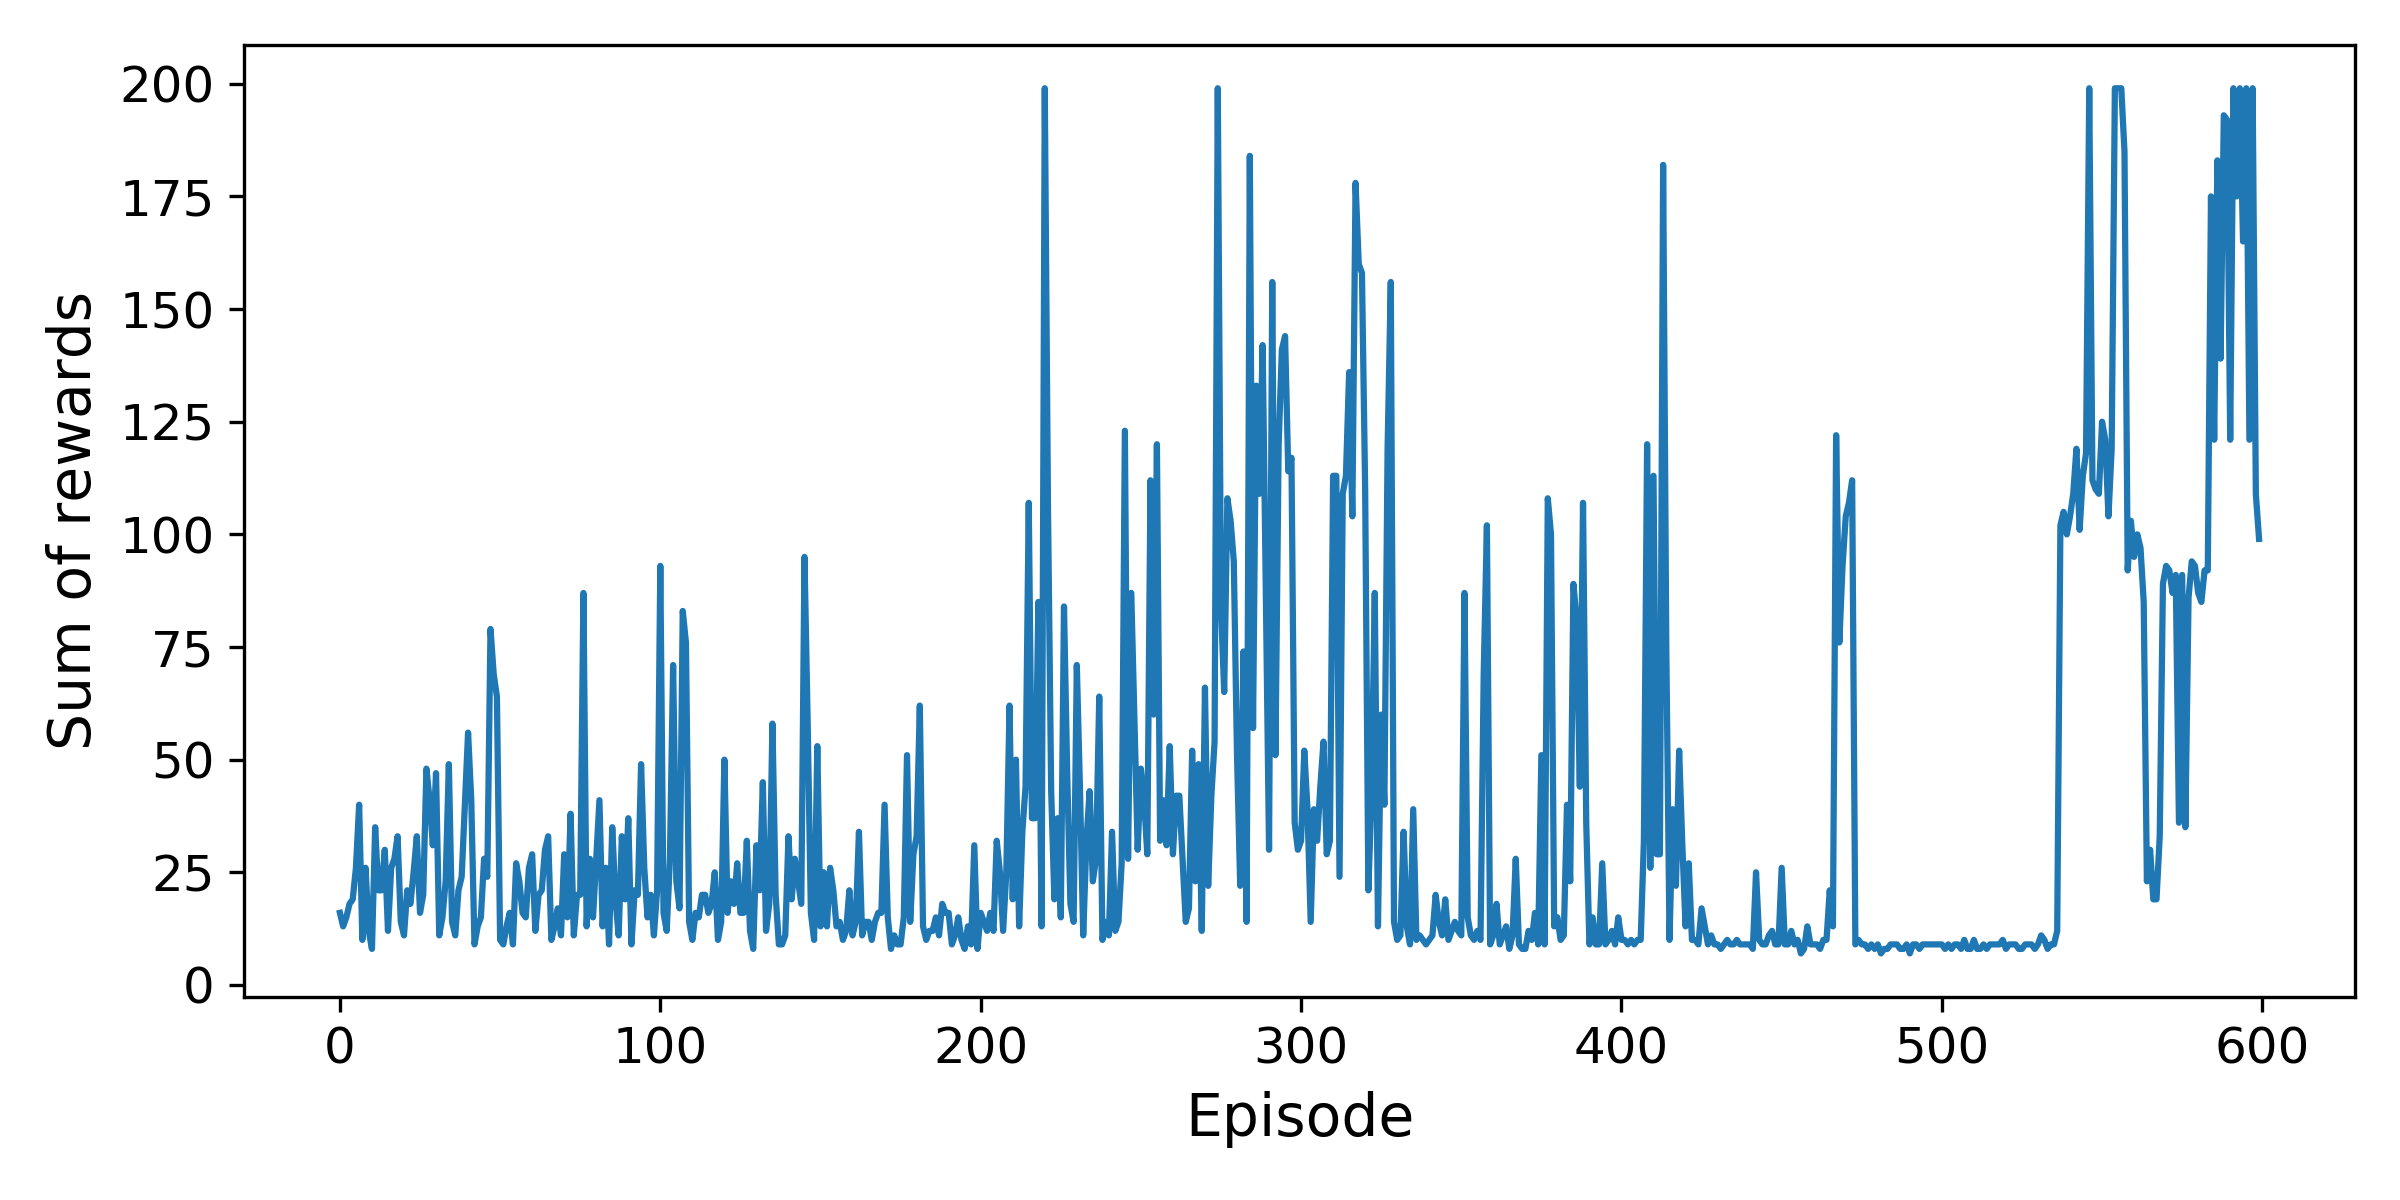
\includegraphics[clip, width=0.8\columnwidth]{figures/rl/dqn_cart_pole_plot.png}
  \end{center}
  
  %\vspace*{-6pt}
  \caption[Learning Curve for Deep Q-Learning on CartPole]{Learning Curve for basic Deep Q-Learning only with simple experience replay on the CartPole environment.}
  \label{fig:learning_curve_dqn}
  %\vspace*{-12pt}
\end{figure}

By defining a loss function we can train our neural network in the same fashion as in supervised learning using the well-known stochastic gradient decent algorithm. This will need thousands or even millions of updates to converge - if it ever does. Deep Q-Learning in its basic form suffers from a lot of problems which results in a DQN learning either slowly, not at all, or suffering from a problem called \textit{catastrophic forgetting}. Figure \ref{fig:learning_curve_dqn} shows the reward over time when solving the CartPole environment. As we can see the agent does not learn anything for 300 episodes, then suddenly achieves the maximum possible reward of 200 and then seems to forget what it has learned. This process then alternates back and forth. Problems like this emerge from a number of different problems:
 \begin{enumerate}
  \item The SGD algorithm assumes that we have data that is \textit{independent and identically distributed} (i.i.d), but our training data is neither independent nor identically distributed. Our samples are generated in episodes which typically make state transitions between states which have a lot in common (e.g. two adjacent frames in a game). Also the distribution of our data is not similar to the distribution the data would have if it has been sampled from an optimal policy. 
  \item We learn from data generated by our current policy (or from a partially random policy in case of $\epsilon$-greedy), which will create samples which are highly correlated. Additionally we use the same model we created our samples with to set our target value and calculate our loss. This may result in a feedback loop which makes training unstable.
  \item In training, the agent will likely overestimate Q-Values. This is due to the nature of the update process. In each step, the target model will select the highest Q-Value, but all Q-Values are estimated. Think of a situation in which each action for a given state has the same Q-Value. An approximation will never be exact, so some of the Q-Values will be slightly higher and some will be slightly lower. When selecting the next Q-Value we do not go for an average we select the highest. Thus we are always prone to overestimation.
 \end{enumerate}

 All these problems combined lead to a very unstable learning process. Fortunately over the years many extensions were developed to reduce their impact dramatically.

\subsection{DQN Extensions} \label{ssec:DQNExtensions}
In this section we want to give a brief overview over techniques that were developed to make Deep Q-Learning more stable. 

\paragraph{Experience Replay.}
At first we want to focus on breaking the correlation between the samples. If we always train from a single episode all our training data will be highly correlated and states will look almost identical. To overcome this instead of learning directly from the trajectory generated by a single episode we introduce a \textit{replay buffer}. After playing an episode we draw random samples from our buffer and learn from them. This will break up the correlation between samples and also reduces the danger of forgetting already learned behavior. On the negative side it introduces new hyperparameters with the size of the replay buffer and the number of samples we want to draw for learning, which are both dependent on the task we are trying to solve. 

\paragraph{Prioritized Experience Replay.}
Lets take the idea of the replay buffer to the next level: Since not all of our samples might be equally important for the learning process, it would be a good idea to replay interesting samples more often than others. This procedure is called \textit{importance sampling} (IS) or \textit{prioritized experience replay} (PIR) and was developed in 2015 by the DeepMind Team \cite{schaul2015prioritized}. The question is what are interesting samples? Schaul et al. proposed to use the TD error term $\delta = r+\gamma V_k(s') - V_k(s)$ (see Section \ref{ssec:TDLearning}) as an indication of a sample being interesting. This makes sense if you think about what a large error means for our algorithm: If we estimated a state value wrong, it is equal to saying we are surprised by the result of the state value. Thus the sample is interesting. \\
In our replay buffer we now assign a priority to each sample, depending on how large the TD error is. We set this priority to a high value for the first time, to ensure that the sample will be sampled at least one time and update the sample priority each time it is sampled to $p = |\delta| + \epsilon$ with $\epsilon$ being a small positive constant to ensure each sample has a non-zero probability of being drawn. A single sample then has the probability of 

\[P(i) = \frac{p_i^\alpha}{\sum_k p_k^\alpha}\]

The exponent $\alpha \in [0, 1]$ is a new hyperparameter which defines how much weight is given to importance sampling with $\alpha = 0$ being standard uniform experience replay.  \\
With some samples being sampled more often than others we again violate our goal of learning uniformly on samples from the target distribution that would be observed if the agent would behave optimally. Without a compensation for this bias, our agent would overfit on those high priority samples. To compensate, we downweight more important samples in training by 

\[w_i = \left(\frac{1}{N} \cdot \frac{1}{P(i)}\right)^\beta\]

where $\beta \in [0, 1]$ is another hyperparameter which controls how much we want to compensate (0 means no compensation). PIR has shown to vastly improve convergence speed and overall performance of Deep Q-Learning, but also introduces two additional hyperparameters which need to be tuned.

\paragraph{Target Networks.}
The next extension aims at improving training stability and reducing the problem of a feedback loop. Since we use the same network to generate samples and to calculate the target Q-Values, situations where training is unstable, diverges or oscillates are very likely. This can be broken up by separating the prediction when generating samples from the calculation of the target values. This is done by working on two similar - but not identical - copies of the same network. We call one of them the \textit{online model} and one the \textit{target model}. The online model will interact with the environment and get updated in the regular update step, while the target model only makes the predictions for the target Q-Value. Every once in a while we copy the weights of the online model to the target model.

\paragraph{Double DQN.}
Next up we want to reduce Q-Value overestimation. This can be done by improving the usage of our target network: Instead of always selecting the action with the highest Q-Value for the Q-target in the update step, we select the action with the highest Q-Value from the online model, and then use the Q-Value estimation for that action from the target DQN. This method was also developed by DeepMind and is called \textit{Double DQN} (DDQN) \cite{van2016deep}.

\paragraph{Dueling DQN.}
Another technique which aims at stabilizing learning is called Duelling DQN \cite{wang2015dueling} (not to be confused with Double DQN). Duelling DQN changes the architecture of the DQN to not compute Q-Values directly, but rather compute two values: The state value $V(s)$ and the so-called \textit{advantage} $A(s, a)$. The advantage expresses how good it is to take an action $a$ in state $s$ in comparison with every other action. The best action $a*$ will have an advantage of 0. Therefore a Q-Value can be expressed as $Q(s, a) = V(s) + A(s, a)$. Computing multiple values which are connected to the same task proves to be beneficial for the training of neural networks and greatly stabilizes training.  %TODO: Source? 

\paragraph{Even more extensions.}
We already discussed a lot of important extensions for Deep Q-Learning, but there are even more. Update steps can be combined into multi-step learning which further stabilizes the training process \cite{sutton1988learning}. Instead of learning to approximate the returns we can also learn to approximate the distribution of returns \cite{bellemare2017distributional}. Like for every neural network the introduction of noise often results in more robust predictions. Additionally the introduction of noise is beneficial in RL because it improves exploration \cite{fortunato2017noisy}. \\

Most of the techniques to improve Deep Q-Learning that were discussed can also be used in conjunction. In 2018 the DeepMind team created an agent which they called \textit{Rainbow} and which was able to outperform all standalone techniques on the Atari 2600 benchmark \cite{hessel2018rainbow}. Even though this proves that the combination of these extensions can be beneficial, the introduction of several new hyperparameters requires careful fine-tuning which might take a lot of time even with modern hyperparametersearch algorithms. %TODO: Make figure for learning with extensions.


\section{Policy Gradient Methods} \label{sec:PGMethods}

\section{Combined Algorithms} \label{sec:CombinedMethods}

\bibliographystyle{abbrv}
\bibliography{sigproc}

\end{document}